\section{Introduction}

Parameter-efficient fine-tuning (PEFT) \citep{houlsby2019adapters,li2021prefix,hu2022lora}
has become a standard approach for adapting large pretrained models.
Over the past several years, a large number of PEFT algorithms have been proposed,
often by modifying a small number of recurring parameterizations.

One major paradigm is the LoRA family, which adapts pretrained weights through
\emph{additive} low-rank updates \citep{hu2022lora}.
Subsequent variants modify how these updates are optimized, scaled, initialized,
or decomposed into magnitude and direction
\citep{hayou2024loraplus,kalajdzievski2023rslora,
wang2024loraga,meng2024pissa,liu2024dora}.
A second paradigm is the OFT family, which adapts weights
\emph{multiplicatively} through structured orthogonal transformations and their
variants \citep{qiu2023oft,qiu2025oftv2,qiu2025poet,yuan2024hra}.
These methods are motivated by seemingly different principles, and many are
presented as principled improvements over vanilla LoRA.
Yet it remains unclear which of these differences survive careful tuning and,
more importantly, which differences matter functionally. This motivates our central question.

\begin{center}
\textbf{\emph{When do typical PEFT methods really differ, and which differences matter?}}
\end{center}

\begin{figure}[t]
\centering
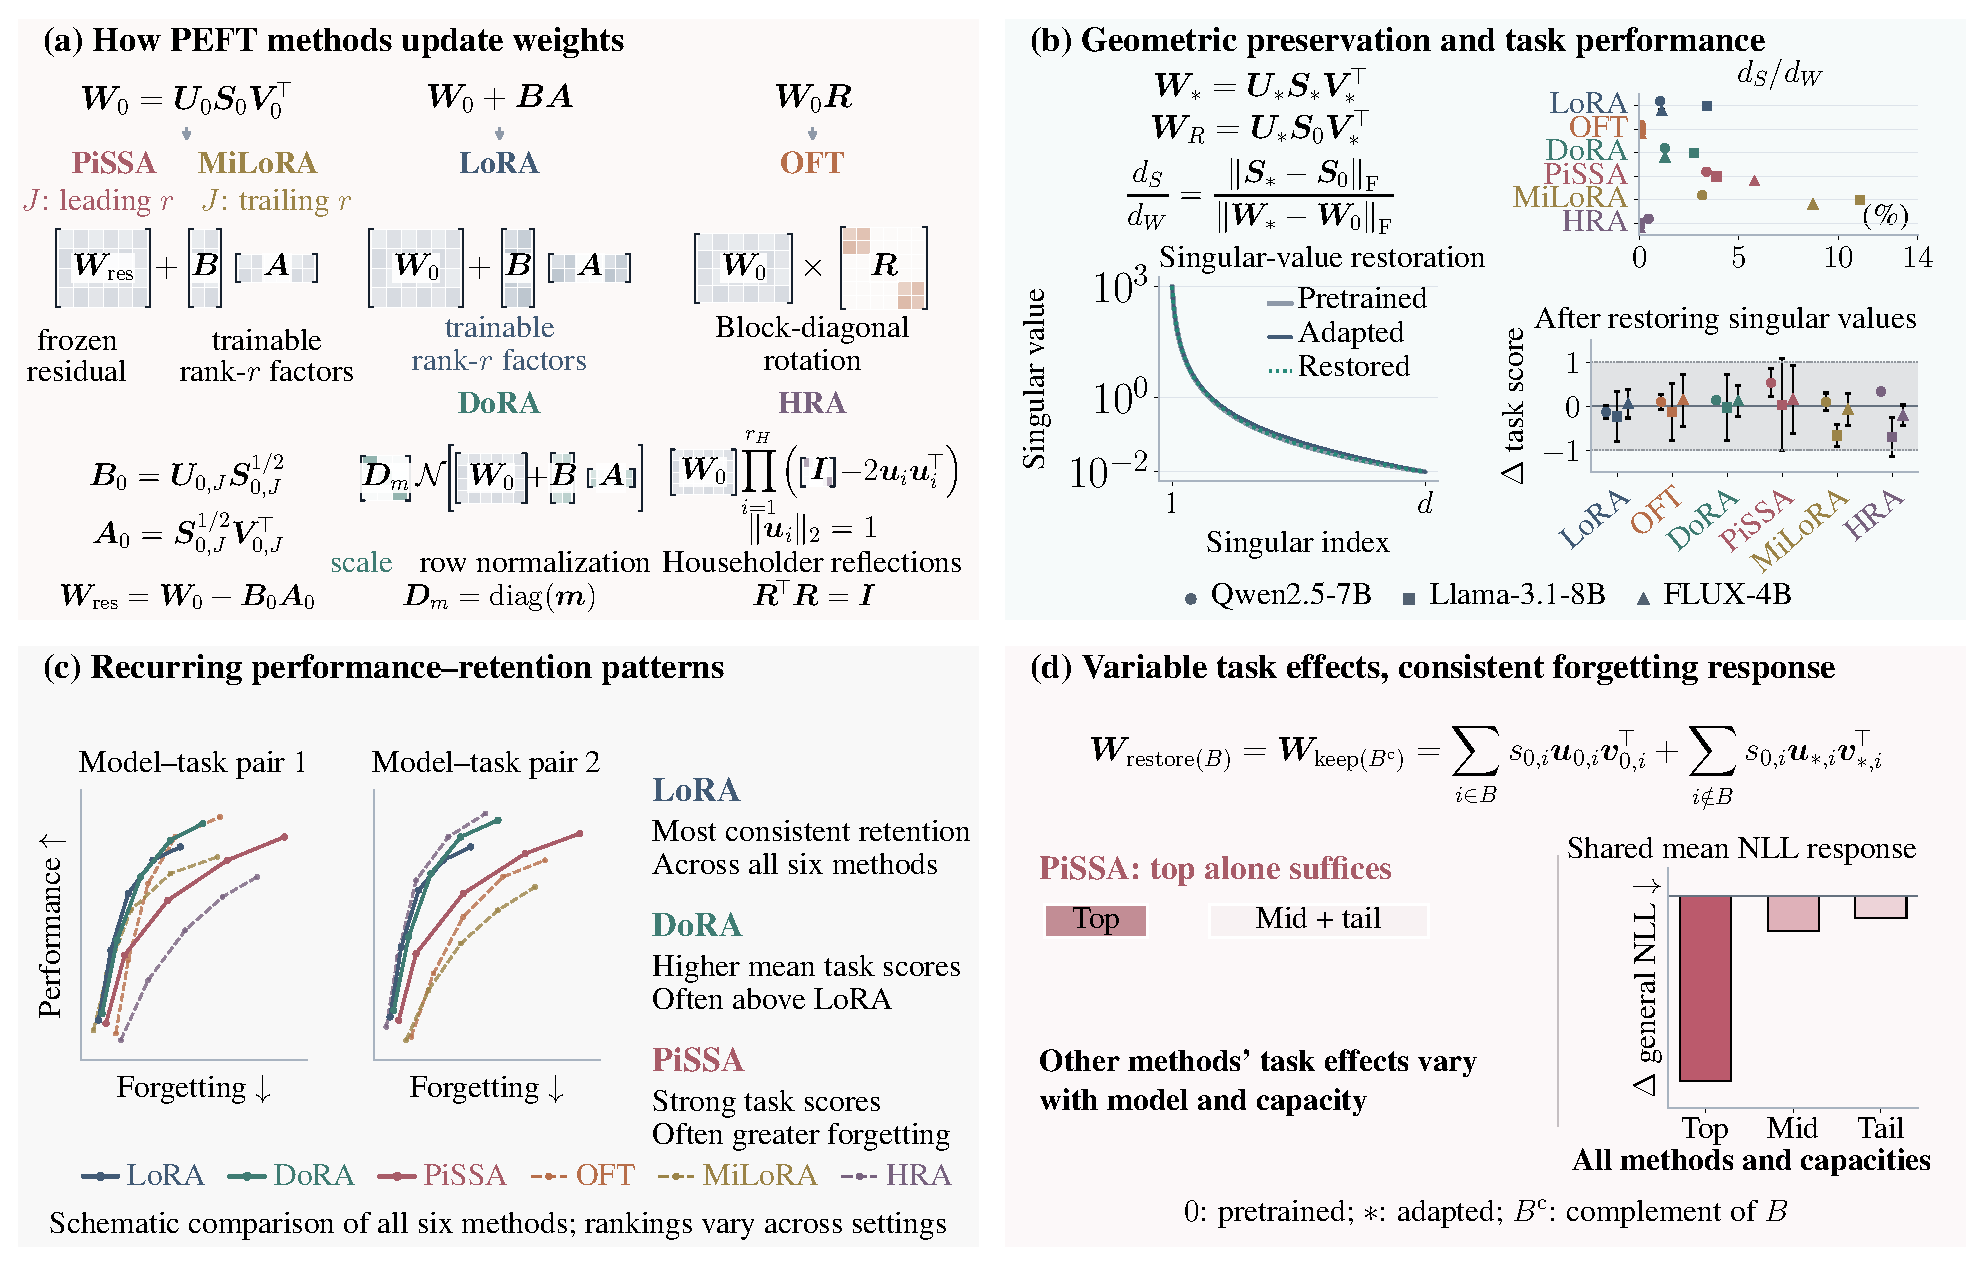
\includegraphics[width=\linewidth]{figures/peft_overview.pdf}
\caption{
Overview of the questions studied in this work.
(a) Six representative PEFT parameterizations.
(b) Changes in pretrained singular spectra and the singular-value restoration
intervention.
(c) Performance and retention comparisons across PEFT methods.
(d) Spectral interventions that selectively retain or restore dominant,
intermediate, and trailing components.
Singular-value decay curves and bar heights are schematic.
}
\label{fig:overview}
\end{figure}

Recent work has begun to question whether apparent methodological improvements
reflect genuinely different operating behavior.
For the LoRA family, \citet{schulman2025lora} identify rescaling invariances
linking initialization scale, update scaling, and factor learning rates, and
show that vanilla LoRA can be highly competitive when properly configured.
\citet{lee2026learningrate} likewise find similar peak performance between
LoRA and its variants after method-specific learning-rate tuning, yet 46 of
64 surveyed studies report a fixed learning rate.
The mathematical-reasoning and image-generation benchmarks in Hugging Face PEFT
\citep[v0.21.0]{mangrulkar2022peft} also report a single training seed and,
for most methods, only one learning-rate setting.
Comparison settings also differ across studies. On GSM8K and MATH, the
main PiSSA comparison adapts all linear layers across three 7B backbones for one
epoch \citep{meng2024pissa}, whereas HRA \citep{yuan2024hra} adapts only
the query and value projections of LLaMA2-7B for two epochs.
These observations motivate common experimental settings, method-specific
tuning and multiple training seeds to separate configuration effects from
methodological gains.

Performance alone, however, may not reveal the full distinction between methods.
Two adapters can achieve similar downstream scores while differing substantially
in how much pretrained behavior they disrupt.
This issue is particularly relevant to orthogonal adaptation.
OFT explicitly preserves hyperspherical geometry
\citep{qiu2023oft}, while HRA connects orthogonal transformations and
low-rank adaptation through Householder reflections \citep{yuan2024hra}.
Such geometric constraints are motivated in part by improved generalization
and preservation of pretrained knowledge
\citep{qiu2023oft,yuan2024hra,huang2026peftarena}.
Two questions remain unresolved.
Do unconstrained LoRA-family methods actually depart substantially from these
geometries in practice? Does tighter geometric preservation translate into
better adaptation or retention?



\subsection{Contributions and findings}

We address these questions by combining controlled empirical comparisons with
direct interventions on pretrained weight geometry.
We also review experimental controls in published PEFT comparisons to guide our study design (\Cref{sec:peft-comparisons}).
We study six representative methods, including LoRA, DoRA, PiSSA, MiLoRA, OFT, and
HRA, across language-model adaptation and diffusion personalization.
Rather than comparing parameterizations only through final task scores, we
examine performance after method-specific tuning, retention of pretrained
capabilities and the functional consequences of the geometric changes they induce.
As summarized in \Cref{fig:overview},
\emph{parameterization labels can overstate geometric differences, whereas
task scores can understate functional differences.}
Our study leads to three main findings.

\noindent {\bf Explicit geometric preservation is not what primarily separates PEFT methods.}
We first characterize adaptation relative to the two-sided orthogonal orbit of
the pretrained weights.
For small isotropically oriented additive updates, the fraction of weight
displacement appearing as singular-value displacement scales as
$1/\sqrt{\max(m,n)}$, showing that limited spectral drift can arise even
without an explicit orthogonality constraint.
Consistent with this prediction, the LoRA-family methods we study exhibit only
modest spectral drift and very small changes in hyperspherical energy.
More importantly, restoring pretrained singular values while retaining the
adapted singular bases largely preserves task performance.
Thus, explicit geometric preservation is neither unique to successful PEFT nor,
in our tested settings, necessary for retaining its task gains.

\noindent {\bf Similar task performance can conceal more persistent differences in retention.}
After method-specific learning-rate tuning, the six methods often achieve
competitive downstream performance, but their retention behavior differs more
systematically.
Across the tested settings, LoRA most consistently limits forgetting while
maintaining competitive performance.
LoRA still has the lowest forgetting in more settings than any other method when learning rates are selected using two seeds and forgetting is measured on the remaining seed, although average rank has exceptions (Appendix~\ref{app:retention-patterns}).
DoRA achieves higher mean task scores than LoRA in most comparisons, typically
with some additional forgetting, whereas PiSSA often incurs larger retention
costs.
Crucially, tighter preservation of pretrained geometry does not reliably
predict better retention.
The more persistent distinctions between methods therefore appear in their
functional consequences, rather than simply in the geometric invariants imposed
by their parameterizations.

\noindent {\bf Adaptation is spectrally heterogeneous, whereas forgetting is spectrally structured.}
We next intervene on dominant, intermediate, and trailing spectral components,
ordered by pretrained singular value.
For task adaptation, there is no universal spectral location of useful change.
PiSSA consistently concentrates task-relevant changes in the dominant
components, whereas for the other methods the sufficient components vary with
the model, capacity, and task.
For forgetting, however, a more consistent pattern emerges.
Restoring the dominant components produces the largest mean reduction in
general-text NLL or base-image drift across all six methods and tested settings.
This ordering persists even in cases where the dominant-component edit is
smaller in norm than alternative edits.
These results suggest that downstream adaptation can be realized through
multiple spectral routes, while forgetting is more consistently coupled to
changes in dominant pretrained components.

Taken together, our results suggest that PEFT methods are better distinguished
by their operating regimes and the functional consequences of learned weight
geometry than by parameterization labels or explicit geometric preservation alone.
